% !TEX TS-program = xelatex
% !BIB program = bibtex
% !TeX spellcheck = ru_RU

% About magic macroses see also
% https://tex.stackexchange.com/questions/78101/

% По умолчанию используется шрифт 14 размера. Если нужен 12-й шрифт, уберите опцию [14pt]
\documentclass[14pt
  , russian
  %, xcolor={svgnames}
  ]{matmex-diploma-custom}
\usepackage[table]{xcolor}
\usepackage{graphicx}
\usepackage{tabularx}
\newcolumntype{Y}{>{\centering\arraybackslash}X}
\usepackage{amsmath}
\usepackage{amsthm}
\usepackage{amsfonts}
\usepackage{amssymb}
\usepackage{mathtools}
\usepackage{thmtools}
\usepackage{thm-restate}
\usepackage{tikz}
\usepackage{wrapfig}
% \usepackage[kpsewhich,newfloat]{minted}
% \usemintedstyle{vs}
\usepackage[inline]{enumitem}
\usepackage{subcaption}
\usepackage{caption}
%\usepackage[nocompress]{cite}
\usepackage{makecell}
% \setitemize{noitemsep,topsep=0pt,parsep=0pt,partopsep=0pt}
% \setenumerate{noitemsep,topsep=0pt,parsep=0pt,partopsep=0pt}


\graphicspath{ {resources/} }

%
% % \documentclass
% %   [ a4paper        % (Predefined, but who knows...)
% %   , draft,         % Show bad things.
% %   , 12pt           % Font size.
% %   , pagesize,      % Writes the paper size at special areas in DVI or
% %                    % PDF file. Recommended for use.
% %   , parskip=half   % Paragraphs: noindent + gap.
% %   , numbers=enddot % Pointed numbers.
% %   , BCOR=5mm       % Binding size correction.
% %   , submission
% %   , copyright
% %   , creativecommons
% %   ]{eptcs}
% % \providecommand{\event}{ML 2018}  % Name of the event you are submitting to
% % \usepackage{breakurl}             % Not needed if you use pdflatex only.
%
% \usepackage{underscore}           % Only needed if you use pdflatex.
%
% \usepackage{booktabs}
% \usepackage{amssymb}
% \usepackage{amsmath}
% \usepackage{mathrsfs}
% \usepackage{mathtools}
% \usepackage{multirow}
% \usepackage{indentfirst}
% \usepackage{verbatim}
% \usepackage{amsmath, amssymb}
% \usepackage{graphicx}
% \usepackage{xcolor}
% \usepackage{url}
% \usepackage{stmaryrd}
% \usepackage{xspace}
% \usepackage{comment}
% \usepackage{wrapfig}
% \usepackage[caption=false]{subfig}
% \usepackage{placeins}
% \usepackage{tabularx}
% \usepackage{ragged2e}
% \usepackage{soul}
\usepackage{csquotes}
% \usepackage{inconsolata}
%
% \usepackage{polyglossia}   % Babel replacement for XeTeX
%   \setdefaultlanguage[spelling=modern]{russian}
%   \setotherlanguage{english}
% \usepackage{fontspec}    % Provides an automatic and unified interface
%                          % for loading fonts.
% \usepackage{xunicode}    % Generate Unicode chars from accented glyphs.
% \usepackage{xltxtra}     % "Extras" for LaTeX users of XeTeX.
% \usepackage{xecyr}       % Help with Russian.
%
% %% Fonts
% \defaultfontfeatures{Mapping=tex-text}
% \setmainfont{CMU Serif}
% \setsansfont{CMU Sans Serif}
% \setmonofont{CMU Typewriter Text}

\usepackage[final]{listings}

\lstdefinelanguage{ocaml}{
keywords={@type, function, fun, let, in, match, with, when, class, type,
nonrec, object, method, of, rec, repeat, until, while, not, do, done, as, val, inherit, and,
new, module, sig, deriving, datatype, struct, if, then, else, open, private, virtual, include, success, failure,
lazy, assert, true, false, end},
sensitive=true,
commentstyle=\small\itshape\ttfamily,
keywordstyle=\ttfamily\bfseries, %\underbar,
identifierstyle=\ttfamily,
basewidth={0.5em,0.5em},
columns=fixed,
fontadjust=true,
literate={->}{{$\to$}}3 {===}{{$\equiv$}}1 {=/=}{{$\not\equiv$}}1 {|>}{{$\triangleright$}}3 {\\/}{{$\vee$}}2 {/\\}{{$\wedge$}}2 {>=}{{$\ge$}}1 {<=}{{$\le$}} 1,
morecomment=[s]{(*}{*)}
}

\lstset{
mathescape=true,
%basicstyle=\small,
identifierstyle=\ttfamily,
keywordstyle=\bfseries,
commentstyle=\scriptsize\rmfamily,
basewidth={0.5em,0.5em},
fontadjust=true,
language=ocaml
}

\newcommand{\cd}[1]{\texttt{#1}}
\newcommand{\inbr}[1]{\left<#1\right>}


\newcolumntype{L}[1]{>{\raggedright\let\newline\\\arraybackslash\hspace{0pt}}m{#1}}
\newcolumntype{C}[1]{>{\centering\let\newline\\\arraybackslash\hspace{0pt}}m{#1}}
\newcolumntype{R}[1]{>{\raggedleft\let\newline\\\arraybackslash\hspace{0pt}}m{#1}}



\usepackage{soul}
\usepackage[normalem]{ulem}
%\sout{Hello World}

% перевод заголовков в листингах
\renewcommand\lstlistingname{Листинг}
\renewcommand\lstlistlistingname{Листинги}

\newcommand{\vsharp}{\textsc{V$\sharp$}}
\newcommand{\fsharp}{\textsc{F$\sharp$}}
\newcommand{\csharp}{\textsc{C$\sharp$}}

\newcommand{\GitHub}{\textsc{GitHub}}
\newcommand{\SMT}{\textsc{SMT}}

\usepackage{afterpage}
\usepackage{pdflscape}

% swapping \phi and \varphi
% https://tex.stackexchange.com/a/50365/171947
\expandafter\mathchardef\expandafter\varphi\number\expandafter\phi\expandafter\relax
\expandafter\mathchardef\expandafter\phi\number\varphi

%https://tex.stackexchange.com/questions/30720/footnote-without-a-marker
\newcommand\blfootnote[1]{%
	\begingroup
	\renewcommand\thefootnote{}\footnote{#1}%
	\addtocounter{footnote}{-1}%
	\endgroup
}

% TODO: Понять, почему я выделил то, что тут в отдельный файл
\usepackage{listings}
\usepackage{tikz}
\usetikzlibrary{decorations.pathreplacing,calc,shapes,positioning,tikzmark}

\newcounter{tmkcount}

\tikzset{
  use tikzmark/.style={
    remember picture,
    overlay,
    execute at end picture={
      \stepcounter{tmkcount}
    },
  },
  tikzmark suffix={-\thetmkcount}
}


\usepackage{comment}
\usepackage{booktabs}%midrule/toprule/...

\usepackage{siunitx} % для таблиц с едлиницами измерений



\usepackage{totcount}

\usepackage{caption}
\usepackage{listings}
%\usepackage{fancyvrb}
\usepackage{fontawesome5}

\DeclareCaptionFont{white}{ \color{white} }
\DeclareCaptionFormat{listing}{
    \parbox{\textwidth}{\hspace{15pt}#1#2#3}
}
\captionsetup[lstlisting]{ format=listing
  %, labelfont=white, textfont=white
  , singlelinecheck=false, margin=0pt, font={bf}
}

\begin{document}
% !TeX spellcheck = ru_RU
% !TEX root = vkr.tex

%% Если что-то забыли, при компиляции будут ошибки Undefined control sequence \my@title@<что забыли>@ru
%% Если англоязычная титульная страница не нужна, то ее можно просто удалить.
\filltitle{ru}{
    %% Актуально только для курсовых/практик. ВКР защищаются не на кафедре а в ГЭК по направлению, 
    %%   и к моменту защиты вы будете уже не в группе.
    chair              = {Кафедра системного программирования},
    group              = {21.Б07-мм},
    %
    %% Макрос filltitle ненавидит пустые строки, поэтому обязателен хотя бы символ комментария на строке
    %% Актуально всем.
    title              = {Автоматизированное построение расписания занятий в вузах на miniKanren},
    % 
    %% Здесь указывается тип работы. Возможные значения:
    %%   coursework - отчёт по курсовой работе;
    %%   practice - отчёт по учебной практике;
    %%   prediploma - отчёт по преддипломной практике;
    %%   master - ВКР магистра;
    %%   bachelor - ВКР бакалавра.
    type               = {practice},
    %
    %% Здесь указывается вид работы. От вида работы зависят критерии оценивания.
    %%   solution - <<Решение>>. Обучающемуся поручили найти способ решения проблемы в области разработки программного обеспечения или теоретической информатики с учётом набора ограничений.
    %%   experiment - <<Эксперимент>>. Обучающемуся поручили изучить возможности, достоинства и недостатки новой технологии, платформы, языка и т. д. на примере какой-то задачи.
    %%   production - <<Производственное задание>>. Автору поручили реализовать потенциально полезное программное обеспечение.
    %%   comparison - <<Сравнение>>. Обучающемуся поручили сравнить несколько существующих продуктов и/или подходов.
    %%   theoretical - <<Теоретическое исследование>>. Автору поручили доказать какое-то утверждение, исследовать свойства алгоритма и т.п., при этом не требуя написания кода.
    kind               = {solution},
    %
    author             = {Габдрахманов Азат Райнурович},
    % 
    %% Актуально только для ВКР. Указывается код и название направления подготовки. Типичные примеры:
    %%   02.03.03 <<Математическое обеспечение и администрирование информационных систем>>
    %%   02.04.03 <<Математическое обеспечение и администрирование информационных систем>>
    %%   09.03.04 <<Программная инженерия>>
    %%   09.04.04 <<Программная инженерия>>
    %% Те, что с 03 в середине --- бакалавриат, с 04 --- магистратура.
    specialty          = {02.03.03 <<Математическое обеспечение и администрирование информационных систем>>},
    % 
    %% Актуально только для ВКР. Указывается шифр и название образовательной программы. Типичные примеры:
    %%   СВ.5006.2017 <<Математическое обеспечение и администрирование информационных систем>>
    %%   СВ.5162.2020 <<Технологии программирования>>
    %%   СВ.5080.2017 <<Программная инженерия>>
    %%   ВМ.5665.2019 <<Математическое обеспечение и администрирование информационных систем>>
    %%   ВМ.5666.2019 <<Программная инженерия>>
    %% Шифр и название программы можно посмотреть в учебном плане, по которому вы учитесь. 
    %% СВ.* --- бакалавриат, ВМ.* --- магистратура. В конце --- год поступления (не обязательно ваш, если вы были в академе/вылетали).
    programme          = {СВ.5006.2019 <<Математическое обеспечение и администрирование информационных систем>>},
    % 
    %% Актуально только для ВКР, только для матобеса и только 2017-2018 годов поступления. Указывается профиль подготовки, на котором вы учитесь.
    %% Названия профилей можно найти в учебном плане в списке дисциплин по выбору. На каком именно вы, вам должны были сказать после второго курса (можно уточнить в студотделе).
    %% Вот возможные вариканты:
    %%   Математические основы информатики
    %%   Информационные системы и базы данных
    %%   Параллельное программирование
    %%   Системное программирование
    %%   Технология программирования
    %%   Администрирование информационных систем
    %%   Реинжиниринг программного обеспечения
    % profile            = {Системное программирование},
    % 
    %% Актуально всем.
    %supervisorPosition = {проф. каф. СП, д.ф.-м.н., проф.}, % Терехов А.Н.
    supervisorPosition = {ассистент кафедры системного программирования}, % Григорьев С.В.
    supervisor         = {Косарев Д.С.},
    % 
    %% Актуально только для практик и курсовых. Если консультанта нет, закомментировать или удалить вовсе.
    %consultantPosition = {должность ООО <<Место работы>> степень}, мое
    %consultant         = {К.~К.~Консультант},мое
    %
    %% Актуально только для ВКР.
    %reviewerPosition   = {должность ООО <<Место работы>> степень}, (М)
    %reviewer           = {Р.~Р.~Рецензент}, (М)
}

% \filltitle{en}{
%     chair              = {Advisor's chair},
%     group              = {ХХ.BХХ-mm},
%     title              = {Template for SPbU qualification works},
%     type               = {practice},
%     author             = {FirstName Surname},
%     % 
%     %% Possible choices:
%     %%   02.03.03 <<Software and Administration of Information Systems>>
%     %%   02.04.03 <<Software and Administration of Information Systems>>
%     %%   09.03.04 <<Software Engineering>>
%     %%   09.04.04 <<Software Engineering>>
%     %% Те, что с 03 в середине --- бакалавриат, с 04 --- магистратура.
%     specialty          = {02.03.03 ``Software and Administration of Information Systems''},
%     % 
%     %% Possible choices:
%     %%   СВ.5006.2017 <<Software and Administration of Information Systems>>
%     %%   СВ.5162.2020 <<Programming Technologies>>
%     %%   СВ.5080.2017 <<Software Engineering>>
%     %%   ВМ.5665.2019 <<Software and Administration of Information Systems>>
%     %%   ВМ.5666.2019 <<Software Engineering>>
%     programme          = {СВ.5006.2019 ``Software and Administration of Information Systems''},
%     % 
%     %% Possible choices:
%     %%   Mathematical Foundations of Informatics
%     %%   Information Systems and Databases
%     %%   Parallel Programming
%     %%   System Programming
%     %%   Programming Technology
%     %%   Information Systems Administration
%     %%   Software Reengineering
%     % profile            = {Software Engineering},
%     % 
%     %% Note that common title translations are:
%     %%   кандидат наук --- C.Sc. (NOT Ph.D.)
%     %%   доктор ... наук --- Sc.D.
%     %%   доцент --- docent (NOT assistant/associate prof.)
%     %%   профессор --- prof.
%     supervisorPosition = {Sc.D, prof.},
%     supervisor         = {S.S. Supervisor},
%     % 
%     consultantPosition = {position at ``Company'', degree if present},
%     consultant         = {C.C. Consultant},
%     %
%     reviewerPosition   = {position at ``Company'', degree if present},
%     reviewer           = {R.R. Reviewer},
% }
\maketitle
\setcounter{tocdepth}{2}
\tableofcontents

% \begin{abstract}
%   В курсаче не нужен
% \end{abstract}

\section*{Введение} %мне к новому году обязательно все
% !TeX spellcheck = ru_RU
% !TEX root = vkr.tex


%цитировать поменьше и записывать 
%``Задачи теории расписаний связаны с построением расписаний, т.е. с упорядочиванием некоторых работ по времени и/или исполнителям с учетом ограничений''~\cite{Алгоритмы}.

В наше время до сих пор остается актуальной проблема составления расписания. В середине прошлого века начался бурный рост теории расписаний ~ \cite{Прорасписание}. Задачи теории расписаний связаны с упорядочиванием некоторых работ по времени и/или исполнителям с учетом ограничений ~\cite{Алгоритмы}.
%``Задачи теории расписаний, разумеется, связаны с построением расписаний, т.е. с упорядочиванием некоторых работ (операций) по
%времени и/или по исполнителям (приборам). При этом необходимо учитывать ограничения на последовательность выполнения работ, ограничения, связанные с исполнителями, и т.п.''~\cite{Алгоритмы}
Одной из задач теории расписаний является задача построения расписания для учебных заведений.

В наше время расписание часто составляется вручную. В предыдущем предложении и далее слово ``расписание'' будет использоваться в контексте расписания для высших учебных заведений. При составлении расписания следует учитывать ряд формальных ограничений, таких как, например, невозможность проводить одному преподавателю два занятия одновременно, невозможность проводить лекционное занятие в обычном классе и другие. Также при составлении расписания желательно учесть и множество других аспектов. Слишком большая кучность занятий увеличивает утомляемость учащихся. Следует учитывать пожелания преподавателей. % попытаться разделить на несколько предложений
% 2 и 3 абзац объединить

 Понятно, что учесть множество этих факторов при составлении расписания вручную можно, но это может быть сопряжено с некоторыми трудностями.Например, если диспетчер расписания на некотором этапе не сможет корректно поставить занятие, то небольшое перестроение расписания может привести к кардинальному изменению всего расписания, что усложняет работу.

%  Также работу диспетчера усложняют, точнее делают ее невозможной, неверные данные, то есть такие данные, по которым составить
% корректное расписание невозможно. Однако выявить, что эти данные
% неверны не так то просто.

% Также важно помнить, что часть задач составления расписания, к которой относится и наша задача, принадлежит классу NP-полных задач ~\cite{ТеорияРасписаний}, которые нельзя решить каким-либо известным полиномиальным алгоритмом.

% ``В настоящий момент широкое распространение имеют метаэвристические алгоритмы, которые находят “хорошее” решение, близкое к оптимальному, за приемлемое время. Недостатком таких алгоритмов является отсутствие оценок качества полученного решения. Неизвестно, насколько решение отличается от оптимального в наихудшем случае''
Задаче составления расписания было уделено внимание со стороны научного сообщества и были разработаны различные методы поиска решения. Учитывая ограничения, включая NP-полноту задачи, хорошо себя показывают эвристические методы, такие как имитация отжига, поиск с запретами, эволюционные алгоритмы ~\cite{Алгоритмы}. Также широкое распространение для решения задач теории расписаний получил метод программирования в ограничениях ~\cite{Алгоритмы}.
% ``При учете всех ограничений, включая NP-полноту задачи, на передний план выходят эвристические методы, такие как имитация отжига, поиск с запретами , эволюционные алгоритмы''~\cite{Алгоритмы}.

% ``В последнее время широкое распространение получил метод программирования в ограничениях (ПвО, в англоязычной литературе – Constraint
% Programming). Одной из областей его успешного применения является
% теория расписаний''~\cite{Прорасписание}. %попытаться сделать меньше ссылок
% % \footnote{Лазарев Александр Алексеевич
% % Гафаров Евгений Рашидович
% % ТЕОРИЯ РАСПИСАНИЙ
% % ЗАДАЧИ И АЛГОРИТМЫ}.
%``Широкое распространение получил метод программирования в ограничениях''~\cite{Прорасписание}. Он довольно успешно применяется для решения задач теории расписаний.

MiniKanren --- семейство встраеваемых языков реляционного программирования, который ранее не использовался при решении данной задачи, если судить по открытым источникам. MiniKanren является языком программирования в ограничениях, поэтому хотелось бы раскрыть потенциал полезного в академическом плане языка при решении практической задачи. В рамках данной работы предлагается разработать решение задачи построения расписания в вузах с помощью языка реляционного программирования miniKanren. 


\blfootnote{
	Дата сборки: \today\\
	
 %\today

\section{Постановка задачи} %обяз
% !TeX spellcheck = ru_RU
% !TEX root = vkr.tex

\label{sec:task}
 Целью работы является создание WEB-приложения с возможностью автоматического построения расписания занятий в вузах с помощью miniKanren со следующими начальными данными:
  \begin{itemize}
 \item  учебный план всех групп;
 \item  количество аудиторий и их специализация;
 \item  данные педагогической нагрузки;
 \item  набор ограничений.
 \end{itemize}
 
 Для её выполнения были поставлены следующие задачи:

 \textbf{Осенний семестр}
 \begin{enumerate}
 %\item Провести обзор аналогов
 \item Разработать процедуру поиска расписания, соответствующего следующим ограничениям:
 \begin{itemize}
         \item учет всех предметов из учебного плана;
 %   \item Вставка не более 5 пар в день
    \item проверка аудиторий на специализацию.
 \end{itemize}
 \item Визуализировать ответ в виде одной общей таблицы с расписанием.
 \end{enumerate}

 \textbf{Весенний семестр}
 \begin{enumerate}
    \item Добавить оценку расписания.
     \item Добавить ограничения:
     \begin{itemize}
         \item полное исключение окон;
    \item нельзя ставить одинокую пару;
    \item проверка аудиторий на вместимость.
 \end{itemize}
    \item Разработать WEB-приложение с возможностью доставать таблицы различных видов и забивать данные не в код.
 \end{enumerate}


\section{Обзор} %обяз
% !TeX spellcheck = ru_RU
% !TEX root = vkr.tex

\label{sec:relatedworks}
% \emph{Обзор должен быть.} Здесь нужно писать, что индустрия и наука уже сделали по вашей теме. Он нужен, чтобы Вы случайно не изобрели какой-нибудь велосипед.

% По-английски называется related works или previous works.

% Если Ваша работа является развитием предыдущей и плохо понимаема без неё, то обзор должен идти в начале. Если же Вы решаете некоторую задачу новым интересным способом, то если поставить обзор в начале, то читатель может устать, пока доберется до вашего решения. В этом случае уместней поставить обзор в конце работы.

% Отечественным аналогом программы для составления расписания является программа:"1c.Автоматическое составление расписания".
% В данной программе составление расписания реализовано в несколких видах
В данном разделе будут рассмотрены готовые продукты для составления расписания.
% \subsection{Обзор методов}
% Задача составления расписания часто встречается в нашей жизни, поэтому ей было уделено немалое внимание со стороны научного сообщества. В данном разделе не будет проводится обзор ручного метода составления расписания, потому что данный метод теряет свою актуальность с каждым днем.
Обзор существующих методов решения задач теории расписания, а не продуктов, можно увидеть в работе~\cite{Прорасписание}.
  \subsection{Обзор решений}
Для автоматического составления расписания реализованы различные решения. В открытом доступе затруднительно найти информацию об алгоритмах составления расписания данных решений. В данном разделе рассмотрим продукты с точки зрения получения расписания. Данные о решениях собраны из различных открытых источников, основной из них ~\cite{Обзоррешение}.
  \begin{itemize}
    \item БИТ.ВУЗ.Расписание.\footnote{https://spb.1cbit.ru/1csoft/bit-vuz-raspisanie/}
    \item 1С:Автоматизированное составление расписания.Университет.\footnote{https://solutions.1c.ru/catalog/asp\_univer/materials}
    \item Экспресс-расписание Колледж.\footnote{https://pbprog.ru/docs/raspis/}
    \item Система «АВТОРасписание».\footnote{https://www.mmis.ru/programs/avtor}
    \item Расписание занятий: «Ректор-Колледж».\footnote{https://rector.spb.ru/}
  \end{itemize}
  Рассмотрим лидирующие в области решения:

\subsubsection{БИТ.ВУЗ.Расписание}
У решения есть полная и ``lite'' версии, рассмотрим полную:\\
% \begin{center}
  % \textbf{Бит.ВузРасписание}
   % \end{center}
  Преимущества данного решения:
  \begin{itemize}
    \item возможность изменять расписание с помощью таблиц;
    \item возможность учесть/игнорировать множество ограничений;
    \item мониторинг ошибок при составлении;
    \item функция составления расписания в смешанном режиме.
  \end{itemize}
  Недостатки:
  \begin{itemize}
      \item возможность составить расписание автоматически только для одной группы за раз;
      %\item Алгоритм составления расписания является жадным
      \item нет возможности использовать бесплатно.
  \end{itemize}
% Реализованные ограничения:
%   \begin{itemize}
%       \item Не более 4 пар в день (и тд, потом написать)
      
%   \end{itemize}

  \subsubsection{1C:Автоматизированное составление расписания}
    Преимущества данного решения:
  \begin{itemize}
    \item возможность изменять расписание с помощью таблиц;
    \item возможность выбора периодичности расписания (неделя,две недели и т.д.);
    \item возможность учесть/игнорировать множество ограничений;
    \item возможность установить ограничения по переходам между корпусами и аудиториями;
    \item мониторинг ошибок при составлении;
    \item функция составления расписания в смешанном режиме;
    \item удобный web-сервис.
  \end{itemize}
  Недостатки:
  \begin{itemize}
      %\item Возможность составить расписание автоматически только для одной группы
     % \item Алгоритм составления расписания является жадным
      \item нет возможности использовать бесплатно;
      \item до покупки затруднительно найти исчерпывающую информацию об алгоритме и о возможностях программы для автоматического построения расписания.
  \end{itemize}
  % Реализованные ограничения:
  % \begin{itemize}
  %     \item Не более 4 пар в день (и тд, потом написать)
  %     \end{itemize}

\textbf{Вывод}

Хотелось бы создать продукт с ясным алгоритмом составления расписания и возможностью составлять расписания на несколько потоков.
\subsection{Используемые инструменты}
\subsubsection{miniKanren} 
Для получения расписания используется miniKanren --- семейство встраеваемых языков реляционного программирования. 

Основные определения и понятия. Более подробную информацию по miniKanren можно увидеть в статье
~\cite{berd}

Программы на miniKanren пишутся с помощью реляций (от англ.``relation'' --- отношение).
Реляция --- вычислимое отношение. 
%miniKanren использует при поиске interliving search.
Ядром miniKanren в языке Racket являются три оператора: $cond^e$ $\equiv$ (введено вместо ==) $fresh$.

$\equiv$ называется унификацией и используется для того, чтобы показать, что два аргумента являются одинаковыми. 
\begin{lstlisting}[caption=Пример применения унификации, language=OCaml, frame=single]
(run 1 (q) ($\equiv$ q 5)) $\implies$ (5) 
(run 1 (q) ($\equiv$ q 5) ($\equiv$ q 6)) $\implies$ () 
\end{lstlisting}
В первой строке программа возвращает (5), но вторая возвращает пустой список, так как нет такого значения q, которое ровно одновременно и 5, и 6.

$cond^e$ зачастую используется для получения нескольких ответов. Рассмотрим применение $cond^e$ на примере.
\begin{lstlisting}[caption=Пример применения $cond^e$, language=OCaml, frame=single]
(run$\infty$ (q) (conde
           [(== q '(matan))];1 ветка
           [(== q '(alg))]; 2 ветка
           [(== q '(geom))]; 3 ветка
           )) $\implies$ ((matan) (alg) (geom))
\end{lstlisting}
Получен ответ ((matan) (alg) (geom)), это означает, что любой из трех списков удовлетворяет реляции $cond^e$. Реляция $cond^e$ ``удовлетворена'', точнее считается завершенной успешно, если успешна завершается хотя бы одна линия $cond^e$. Также стоит обратить внимание на порядок вывода ответов, $cond^e$ выполняет ветки по порядку их написания.

$fresh$ используется для создания свежих переменных
\begin{lstlisting}[caption=Использование $fresh$ и унификации, language=OCaml, frame=single]
(run 1 (q) (fresh (x y) ($\equiv$ x y) ($\equiv$ x 3) ($\equiv$ y q))) $\implies$ (3)
\end{lstlisting}
Таким образом, в данной программе x, y и q равны 3 и переменные перестают быть свежими, теперь попытка унификации любой из переменных с любым значение, кроме 3, приведет к пустому выводу программы.



%Особенностью miniKanren является то, что программы на нем пишутся с помощью реляций (от англ.``relation'' --- отношение).
%это функция, в которой нет различия между входными и выходными данными и которая "связывает", то есть задает некоторое отношение между переменными.


% Как упоминалось, наша задача принадлежит классу NP-полных задач.
% %( Алгоритма, для гарантированного поиска корректного расписания нет)!!!!! ОЧень сильное высказывание.
% MiniKanren, используя interliving search, имеет возможность найти ответы за разумное время.
%Лучшим вариантом для составления расписания является метод "ветвей и границ", который и использует miniKanren при поиске ответа.\\


Выбрана каноническая реализация miniKanren на Racket \\``faster-miniKanren''~\cite{faster}


\subsubsection{Racket\footnote{https://racket-lang.org/}}
Так как выбрана реализация miniKanren на Racket, и для оценки результата требуется лишь визуализация в виде общей таблицы, то было решено не включать дополнительных технологий в работу и использовать язык Racket для визуализации.




% \section{Используемые инструменты}
% \subsection{miniKanren} 
Для получения расписания по начальным данным использован miniKanren --- представитель семейства языков реляционного программирования. Особенностью miniKanren является то, что программы на нем пишутся с помощью реляций. Где реляция это функция, в которой нет различия между входными и выходными данными.


Как упоминалось, наша задача принадлежит классу NP-полных задач.
%( Алгоритма, для гарантированного поиска корректного расписания нет)!!!!! ОЧень сильное высказывание.
miniKanren, используя поиск в ширину, имеет возможность найти ответы за разумное время.
%Лучшим вариантом для составления расписания является метод "ветвей и границ", который и использует miniKanren при поиске ответа.\\


Выбрана каноническая реализация miniKanren на Racket ``faster-miniKanren''~\cite{faster}


\subsection{Racket}
Так как выбрана реализация miniKanren на Racket, и для оценки результата требуется лишь визуализация в виде общей таблицы, то было решено не включать дополнительных технологий в работу и использовать язык Racket для визуализации.


% \section{Background (опционально)}
% Здесь пишется некоторая дополнительная информация о том, зачем делается то, что делается.

% Например, в работе придумывается какой-то новый метод решения формул в \SMT{} в теориях с числами. Без каких-то дополнительных пояснений будет казаться, что работа состоит из жестокого ``матана'' и совсем не по теме кафедры системного программирования. 
% Поэтому, в данном разделе стоит рассказать, что все эти методы примеряются для верификации в проекте \vsharp{}, и поэтому непосредственно связаны с тематикой кафедры.


%\section{Метод}
%% !TeX spellcheck = ru_RU
% !TEX root = vkr.tex

%Реализация в широком смысле: что таки было сделано. Скорее всего самый большой раздел.

%\emph{Крайне желательно} к Новому году иметь что-то, что сюда можно написать.

% Для понимания того как курсовая записка (отзыв по учебной практике/ВКР) должна писаться, можно посмотреть видео ниже. Они про научные доклады и написание научных статей, учебные практики и ВКР отличаются тем, что тут есть требования отдельных глав (слайдов) со списком задач и списком результатов. Но даже если вы забьёте не требования специфичные для ВКР, и соблюдете все рекомендации ниже, получившиеся скорее всего будет лучше чем первая попытка 99\% ваших однокурсников.
\subsection{Алгоритм}
Реализация представляет из себя пошаговое построение расписание для всех групп по порядку. Мы имеем группу, учебный план и преподавателей,"привязанных" к определенному предмету. Мы берем первый предмет из учебного плана, расписание самой группы, расписание преподавателя и расписание первой попавшейся аудитории, в которой возможно провести данный предмет. После чего мы пытаемся вставить этот предмет в расписание группы, преподавателя и аудитории в одну из пар с понедельника по пятницу. Если это получается, то идем дальше, если не получается, то мы берем уже другую аудиторию, где можно провести данное занятие и повторяем процедуру. Далее или на каком-то этапе у нас получается поставить пару, или мы, перебрав все аудитории, так и не смогли поставить пару. В первом случае мы заканчиваем данный шаг и берем следующий предмет и следующего преподавателя, в противом же случае у нас расписание несоставимо, значит miniKanren сам "откатывается" назад на один шаг и продолжает попытки.                            (очень душно написал, это просто нечитаемо)                       
\subsection{Реализация ограничений}
\textbf{Реализованы следующие ограничения:}
\begin{enumerate}
    \item Учет всех предметов из учебного плана
    \item Вставка не более 5 пар в день
    \item Проверка аудиторий на вместимость и на их специализацию
  %  \item Невозможность поставить только одну пару в день в расписание
\end{enumerate}

\subsubsection{Учет всех предметов из учебного плана}
Реализация данного ограничения является наиболее трудоемкой частью работы, ведь именно на основе этого ограничения и строится алгоритм. Сложность - лучшим образом расставить конъюнкты, чтобы расписание составлялось максимально быстро.

\subsubsection{Не более 5 пар в день}
Для данного ограничения реализована реляция проверки каждого дня на количество пар

\subsubsection{Проверка аудиторий}
Проверка аудиторий происходит по ходу алгоритма, на каждом шаге все аудитории используются только по назначению и в пределах вместимости.

% \begin{enumerate}
% \item <<Как сделать великолепный научный доклад>> от Саймона Пейтона Джонса~\cite{SPJGreatTalk} (на английском).
% \item <<Как написать великолепную научную статью>> от Саймона Пейтона Джонса~\cite{SPJGreatPaper} (на английском).
% \item <<Как писать статьи так, чтобы люди их смогли прочитать>> от Дэрэка Драйера~\cite{DreyerYoutube2020} (на английском). По предыдующей ссылке разбираются, что должно быть в статье, т.е. как она должна выглядеть на высоком уровне. Тут более низкоуровнево изложено как должны быть устроены параграфы и т.п.
% \item Ещё можно посмотреть <<How to Design Talks>>~\cite{JhalaYoutube2020} от Ranjit Jhala, но я думаю, что первых трех ссылок всем хватит.
% \end{enumerate}


% \subsection{Основные грабли}
% Здесь мы будем собирать основные ошибки, которые случаются при написании текстов. В интернетах тоже можно найти коллекции типичных косяков\footnote{\href{https://www.read.seas.harvard.edu/~kohler/latex.html}{https://www.read.seas.harvard.edu/~kohler/latex.html}}.


% \begin{lstlisting}[caption=Название обязательно, language=Caml, frame=single]
% let x = 5 in x+1
% \end{lstlisting}

% Рекомендуется использовать красивые греческие буквы $\Phi,\phi$ по-умол\-ча\-нию, а именно $\phi$ вместо $\varphi$. В данном шаблоне команды для этих букв переставлены местами по сравнению с ванильным \TeX'ом.


% \subsection{Выделения куска листинга с помощью tikz}            
% \url{https://tex.stackexchange.com/questions/284311}

% \begin{lstlisting}[escapechar=!,basicstyle=\ttfamily]
% #include <stdio.h>
% #include <math.h>

% int main () {
%   double c=-1;
%   double z=0;
%   int i;

%   printf (``For c = %lf:\n'', c );
%   for ( i=0; i<10; i++ ) {
%     printf ( !\tikzmark{a}!"z %d = %lf\n"!\tikzmark{b}!, i, z );
%     z = pow(z,2) + c;
%   }
% }
% \end{lstlisting}

% \begin{tikzpicture}[use tikzmark]
% \draw[fill=gray,opacity=0.1]
%   ([shift={(-3pt,2ex)}]pic cs:a) 
%     rectangle 
%   ([shift={(3pt,-0.65ex)}]pic cs:b);
% \end{tikzpicture}



% \section{Эксперимент (желательно к Новому году)}
% % !TeX spellcheck = ru_RU
% !TEX root = vkr.tex

Как мы проверяем, что  всё удачно получилось.  К Новому году для промежуточного отчета желательно хотя бы описать как он будет проводиться и на чем. (Предполагаю/ что сюда нужно будет написать хотя бы что-нибудь по поводу проблем / которые встречаются при написании кода:примером может послужить хотя бы ситуация/ когда меняются конъюнкты местами)

\subsection{Условия эксперимента}
Железо (если актуально);  версии ОС, компиляторов и параметры командной строки; почему мы выбрали именно эти тесты; входные данные, на которых проверяем наш подход, и почему мы выбрали именно их.

\subsection{Исследовательские вопросы (Research questions)}
Надо сформулировать то, чего мы хотели бы добиться работой (2 штуки будет хорошо):

\begin{itemize}
\item Хотим алгоритм, который лучше вот таких-то остальных.
\item Если в подходе можно включать/выключать составляющие, то насколько существенно каждая составляющая влияет на улучшения.
\item Если у нас строится приближение каких-то штук, то на сколько точными будут эти приближения.
\item и т.п.
\end{itemize}

Иногда в работах это называют гипотезами, которые потом проверяют. Далее в тексте можно ссылаться на research questions как \textsc{RQ}, это общепринятое сокращение.

\subsection{Метрики}

Как мы сравниваем, что результаты двух подходов лучше или хуже:
\begin{itemize}
\item Производительность.
\item Строчки кода.
\item Как часто алгоритм "угадывает" правильную классификацию входа.
\end{itemize}

Иногда метрики вырожденные (да/нет), это не очень хорошо, но если в области исследований так принято, то ладно.

\subsection{Результаты}
Результаты понятно что такое. Тут всякие таблицы и графики, как в таблице \ref{time_cmp_obj_func}. Обратите внимание, как цифры выровнены по правому краю, названия по центру, а разделители $\times$ и $\pm$ друг под другом. 

Скорее всего Ваши измерения будут удовлетворять нормальному распределению, в идеале это надо проверять с помощью критерия Колмогорова и т.п. Если критерий этого не подтверждает, то у Вас что-то сильно не так с измерениями, надо проверять кэши процессора, отключать Интернет во время измерений, подкручивать райнтайм, чтобы сборка мусора не вмешивалась и т.п. Если критерий удовлетворён, то необходимо либо указать мат. ожидание и доверительный/предсказывающий интервал, либо написать, что все измерения проводились с погрешностью, например, в 5\%. Замечание: если у вас получится улучшение производительности в пределах погрешности, то это обязательно вызовет вопросы.

В этом разделе надо также коснуться Research Questions.

\subsubsection{RQ1} Пояснения
\subsubsection{RQ2} Пояснения

\begin{table}
\def\arraystretch{1.1}  % Растяжение строк в таблицах
\setlength\tabcolsep{0.2em}
\centering
% \resizebox{\linewidth}{!}{%
    \caption{Производительность какого-то алгоритма при различных разрешениях картинок  (меньше --- лучше), в мс.,  CI=0.95. За пример таблички кидаем чепчики в честь Я.~Кириленко}
    \begin{tabular}[C]{
    |S[table-format=4.4,output-decimal-marker=\times]
    *4{|S
          [table-figures-uncertainty=2, separate-uncertainty=true, table-align-uncertainty=true,
          table-figures-integer=3, table-figures-decimal=2, round-precision=2,
          table-number-alignment=center]
          }
    |}
    \toprule
        \multicolumn{1}{|c|}{Resolution} & \multicolumn{1}{c|}{\textsc{TENG}} & \multicolumn{1}{c|}{\textsc{LAPM}} &
        \multicolumn{1}{|c|}{\textsc{VOLL4}} \\ \hline
        1920.1080 & 406.23 \pm 0.94 & 134.06 \pm 0.35 & 207.45 \pm 0.42  \\ \hline
        1024.768  & 145.0 \pm 0.47  & 39.68 \pm 0.1   &  52.79  \pm 0.1 \\ \hline
        464.848   & 70.57 \pm 0.2   & 19.86 \pm 0.01     & 32.75  \pm 0.04 \\ \hline
        640.480   & 51.10 \pm 0.2   & 14.70 \pm 0.1 & 24  \pm 0.04 \\ \hline
        160.120   & 2.4 \pm 0.02    & 0.67 \pm 0.01      & 0.92  \pm 0.01 \\
        \bottomrule
    \end{tabular}%
%}
    \label{time_cmp_obj_func}
\end{table}

\clearpage
% !TeX spellcheck = ru_RU
% !TEX root = vkr.tex

\newcolumntype{C}{ >{\centering\arraybackslash} m{4cm} }
\newcommand\myvert[1]{\rotatebox[origin=c]{90}{#1}}
\newcommand\myvertcell[1]{\multirowcell{5}{\myvert{#1}}}
\newcommand\myvertcelll[1]{\multirowcell{4}{\myvert{#1}}}
\newcommand\myvertcellN[2]{\multirowcell{#1}{\myvert{#2}}}


\afterpage{%
    \clearpage% Flush earlier floats (otherwise order might not be correct)
    \thispagestyle{empty}% empty page style (?)
    \begin{landscape}% Landscape page
        \centering % Center table

\begin{tabular}{|c|c|c|c|c|c|c|c|c|c|c|c|c|c|c|c|c|c|}\hline
%& \multicolumn{17}{c|}{} \\ \hline 
\multirowcell{2}{Код модуля \\в составе \\ дисциплины,\\практики и т.п. }
  &\myvertcellN{2}{Трудоёмкость}
  & \multicolumn{10}{c|}{\tiny{Контактная работа обучающихся с преподавателем}} 
  & \multicolumn{5}{c|}{\tiny{Самостоятельная работа}} 
  & \myvertcellN{2}{\tiny Объем активных и интерактивных } 
  \\ \cline{3-17}

&& \myvertcellN{2}{лекции} 
    &\myvertcellN{2}{семинары}
    &\myvertcellN{2}{консультации}
    &\myvertcellN{2}{\small практические  занятия }
    &\myvertcellN{2}{\small лабораторные работы }
    &\myvertcellN{2}{\small контрольные работы }
    &\myvertcellN{2}{\small коллоквиумы }
    &\myvertcellN{2}{\small текущий контроль }
    &\myvertcellN{2}{\small промежуточная аттестация }
    &\myvertcellN{2}{\small итоговая аттестация }
    
    &\myvertcellN{2}{\tiny под руководством    преподавателя}
    &\myvertcellN{2}{\tiny в присутствии     преподавателя   }
    &\myvertcellN{2}{\tiny с использованием    методических}
    &\myvertcellN{2}{\small текущий контроль}
    &\myvertcellN{2}{\tiny промежуточная аттестация } 
    &     \\
&& &&&&&&&&& &&&&&&\\
&& &&&&&&&&& &&&&&&\\
&& &&&&&&&&& &&&&&&\\ 
&&&&&&&&&&& &&&&&&\\ 
&&&&&&&&&&& &&&&&&\\ 
&&&&&&&&&&& &&&&&&\\ \hline
Семестр 3 & 2 &30  &&&&&&&&2   & &&&18 &&20 &10\\ \hline
          &   &2-42&&&&&&&&2-25& &&&1-1&&1-1&\\ \hline
Итого     & 2 &30  &&&&&&&&2   & &&&18 &&20 &10\\ \hline
\end{tabular}

        \captionof{table}{Если таблица очень большая, то можно её изобразить на отдельной портретной странице}
    \end{landscape}
    \clearpage% Flush page
}



\subsection{Обсуждение результатов}

Чуть более неформальное обсуждение, то, что сделано. Например, почему метод работает лучше остальных? Или, что делать со случаями, когда метод классифицирует вход некорректно. 



% \section{Применение (того, что сделано на практике)}

% Если применение в лоб не работает, потому что всё изложено чуть более сжато и теоретично, надо рассказать тонкости и правильный метод применения результатов. Если результаты применяются без дополнительных телодвижений, то про это можно не писать.

% \section{Угрозы нарушения корректности (опциональный)}

% Если основная заслуга метода, это то, что он дает лучшие цифры, то стоит сказать, где мы могли облажаться, когда
% \begin{enumerate}
% \item проводили численные замеры;
% \item выбирали тестовый набор (см. \emph{confirmation bias})
% \end{enumerate} 




\section{Реализация}
\subsection{Реализация поиска расписания, соответствующего требованиям}
Вся сложность реализации данного пункта заключается в том, что нужно сделать поиск расписания максимально быстрым, для этого нужно оптимальным способом закодировать в miniKanren поставленные ограничения.
\begin{itemize}
    \item Учет всех предметов из учебного плана
   % \item Не более 6 пар в день
    \item Проверка аудиторий
\end{itemize}
\subsubsection{Учет всех предметов из учебного плана}
Особенностью miniKanren является то, что при составлении запроса важен порядок конъюнктов.
Таким образом, нужно понять, при каком порядке запрос будет завершен быстрее всего. Так как поиск происходит в ширину, то нужно дать возможность программе понять, на каком моменте нужно "обломить" ветку.

\textbf{Важные частные случаи:}
\begin{enumerate}
    \item Обычно группы более "заняты", чем преподаватели, то есть вероятность зайти в тупиковую ветвь быстрее через группу выше. Поэтому конъюнкт, который отвечает за вставку предмета в группу, ставится раньше, чем конъюнкт, отвечающий за преподавателя
    \item При составлении расписания пытаются если задействовать аудиторию, то сделать это по максимуму, поэтому стоит конъюнкт с вставкой предмета ставить спереди преподавателя. 
  % \textbf{Пример вставки предмета с помощью унификации} 
   \begin{lstlisting}[caption=Использование унификации для вставки 4 пары, language=OCaml, frame=single]
    (define (sched subj teachersched schedgroup
     schedclass)
    (fresh (a1 a2 b1 b2 c1 c2)
    (== teachersched `(,a1 . ,a2)) (== a2 subj)
    (== schedgroup `(,b1 . ,b2)) (== b2 subj)
    (== schedclass `(,c1 . c2)) (== c2 subj)))
\end{lstlisting}
    Данная реляция завершается успешно, если получается выполнить все три действия, в противном случае она завершается неуспешно и вызывается другая реляция, которое делает то же самое, просто пытается вставить предмет на другую пару или день.
\end{enumerate}

% \subsubsection{Не более 6 пар в день}
% Данное ограничение решается сразу с помощью двух приемов 
% \begin{itemize}
%     \item Линии conde, которые отвечают за 6 пары, стоят в самом конце, что означает, что предмет вставлен будет на 6 пару только тогда, когда иного варианта нет. Но если окажется, что при вставке 6 пары день будет забит полностью, то сработает реляция, которая показана в следующем пункте
%     \item Реляция =/=, входящая в ядро faster-minikanren. 
%     \begin{lstlisting}[caption=Использование \neq, language=Racket, frame=single]
%     (define (checkfivesubj schedgroup)
%     (fresh (a1 a2 a3 a4 a5 a6)
%     (=/= schedgroup `(,a1,a2,a3,a4,a5,a6))))
% (checkfivesubj schedgroup)
%     \end{lstlisting}
%     Был испробован вариант с использованием реляции lenghto, которая связывает список и длину списка, но данная реляция замедляет код.
% \end{itemize}

\subsubsection{Проверка аудиторий}
За каждой аудиторией закреплено множество предметов, которые могут в ней проводится.
На каждом этапе, когда нужно поставить предмет в расписание, мы должны взять аудиторию, которая подходит для этого. \\
Наиболее удобной реляцией для проверки возможности проведения предмета является $member^o$, которая проверяет, является ли частью списка некоторый элемент, в нашем случае она проверяет, входит ли предмет в список предметов проводимых в аудитории.


\subsection{Дополнительные возможности}

   \subsubsection{Мнение преподавателя} По желанию преподавателя можно освобождать ему определенную пару или день. Время работы программы зачастую почти не меняется, при освобождении или занятии пары, но в некоторых ситуациях эти изменения могут сильно повлиять время ответа, причем в любую сторону.
   
   Реализована данная возможность с помощью реляции унификации: Взяв определенный день или пару расписания, унифицируем переменную, отвечающую за этот день или пару, с пустым списком.
   
   \subsubsection{Освободить определенное время}. Возможность освободить определенные пары у группы. Реализовано аналогично предыдущему пункту.
   \subsubsection{Кучность} Возможность "сдвигать" пары относительно дней недели или номера пар. То есть сдвигать пары в сторону понедельника или в сторону 2-4 пары. 
 %  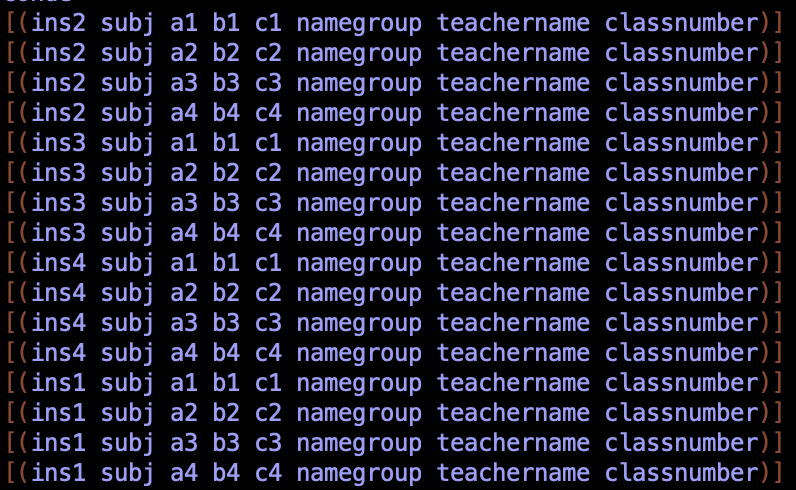
\includegraphics[width=0,5\textwidth]{condeline.png}
   Специально для этой возможности было написано 20 различных линий conde, где каждая линия отвечает за вставку предмета в определенный день и пару. При изменении порядка линий conde, будет меняться "сдвиг" предметов в пределах недели.
  \begin{lstlisting}[caption=Сдвиг пар, language=OCaml, frame=single]
[(ins2 subj a1 b1 c1 namegroup teachername classnumber)]
[(ins2 subj a2 b2 c2 namegroup teachername classnumber)]
[(ins2 subj a3 b3 c3 namegroup teachername classnumber)]
[(ins2 subj a4 b4 c4 namegroup teachername classnumber)]
[(ins2 subj a5 b5 c5 namegroup teachername classnumber)]
\end{lstlisting}
Представлено 5 линий conde, каждая из которых отвечает за вставку второй пары в определенный день, меняя их местами кучность будет меняться.




% \subsection{Дальнейшие улучшения}
% Добавление следующих ограничений включает в себя погружение в потроха minikanren. 

% \subsubsection{Отсутствие окон}
% Пока не реализовано решение для провеки на окна, используется следующий способ для минимизации окон для первого курса: так как поиск расписания происходит в ширину, то, вызвав в первую очередь составление расписания для первых курсов, там самым мы гарантируем кучность пар для них. 
% \subsubsection{Одинокая пара}
% В данном случае сложно прогнозировать поведение miniKanrena, поэтому есть вероятность постановки одинокой пары, но, чаще всего, это происходит не более раза.
% \subsection{Дополнительные возможности}
% \begin{itemize}
%     \item По желанию преподавателя можно или оставлять свободной какую-либо пару или день, или гарантированно вставить в нее занятие.
%     \item Возможность занять определенные пары у группы или освободить
%     \item Возможность "сдвигать" пары относительно дней недели или номера пар. То есть сдвигать пары в сторону понедельника или в сторону 2-4 пары. 
% \end{itemize}
\subsection{Визуализация}
Визуализация реализована с помощью библиотеки ``simple-xlsx''~\cite{symple}
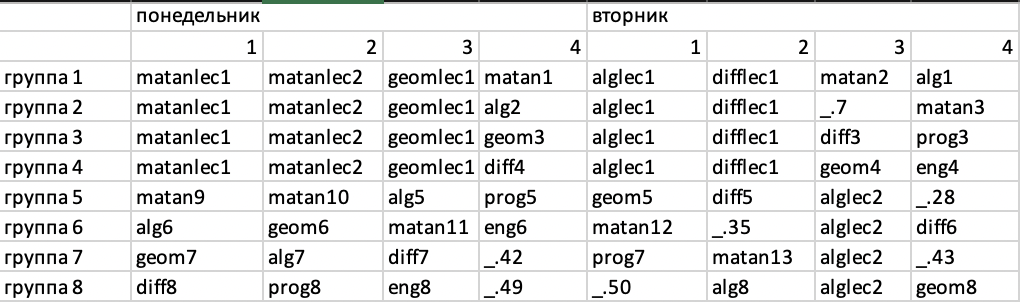
\includegraphics[width=1\textwidth]{sched.png}

% \subsection{Дополнительные возможности}
% \begin{itemize}
%     \item По желанию преподавателя можно или оставлять свободной какую-либо пару или день, или гарантированно вставить в нее занятие.
%     \item Возможность занять определенные пары у группы или освободить
%     \item Возможность "сдвигать" пары относительно дней недели или номера пар. То есть сдвигать пары в сторону понедельника или в сторону 2-4 пары. 
% \end{itemize}

\section{Замеры производительности}

  
    %здесь создаю табличку с вариантами тестов, с количеством ответов и временем еще можно с одинаковыми данными забить по разному запросы (разделить или соединить)
Замеры проводятся на ноутбуке MacBook Air 13 M1, 8 Gb RAM.\\
Расписание строилось на два потока, в каждом из которых по 4 группы. Учебный план групп был создан на основе плана направления ``Технологии программирования''.

%      \begin{tabbing}
%  \hspace{6em}\= \hspace{12em}\= 
% \hspace{6em}\kill
%  № \> Количество запросов \> Время \\
%  1 \> 2 \> 60 \\
%  2 \> 10 \> 72 \\
%  3 \> 200 \>  90
%     \end{tabbing}

%     \begin{table}
% \caption{Замеры тестов на два потока}
% %\label{tabular}
% %\begin{center}
% \begin{tabular}{ccc}
% № & Количество ответов & время, сек. \\%почему то при объединении не работает вовсе, можно попробовать работать с отдельно вызываемыми функциями
% 1 & 2 & 60\\
% 2 & 10 & 72 \\
% 3 & 200 & 90 \\
% \end{tabular}
% %\end{center}
% \end{table}
 Довольно малое увеличение времени работы алгоритма для получения большего количества расписаний обусловлено тем, что miniKanren использует поиск в ширину. Данный факт можно использовать для получения большого количества расписаний и выбора из них "наиболее удобного".

%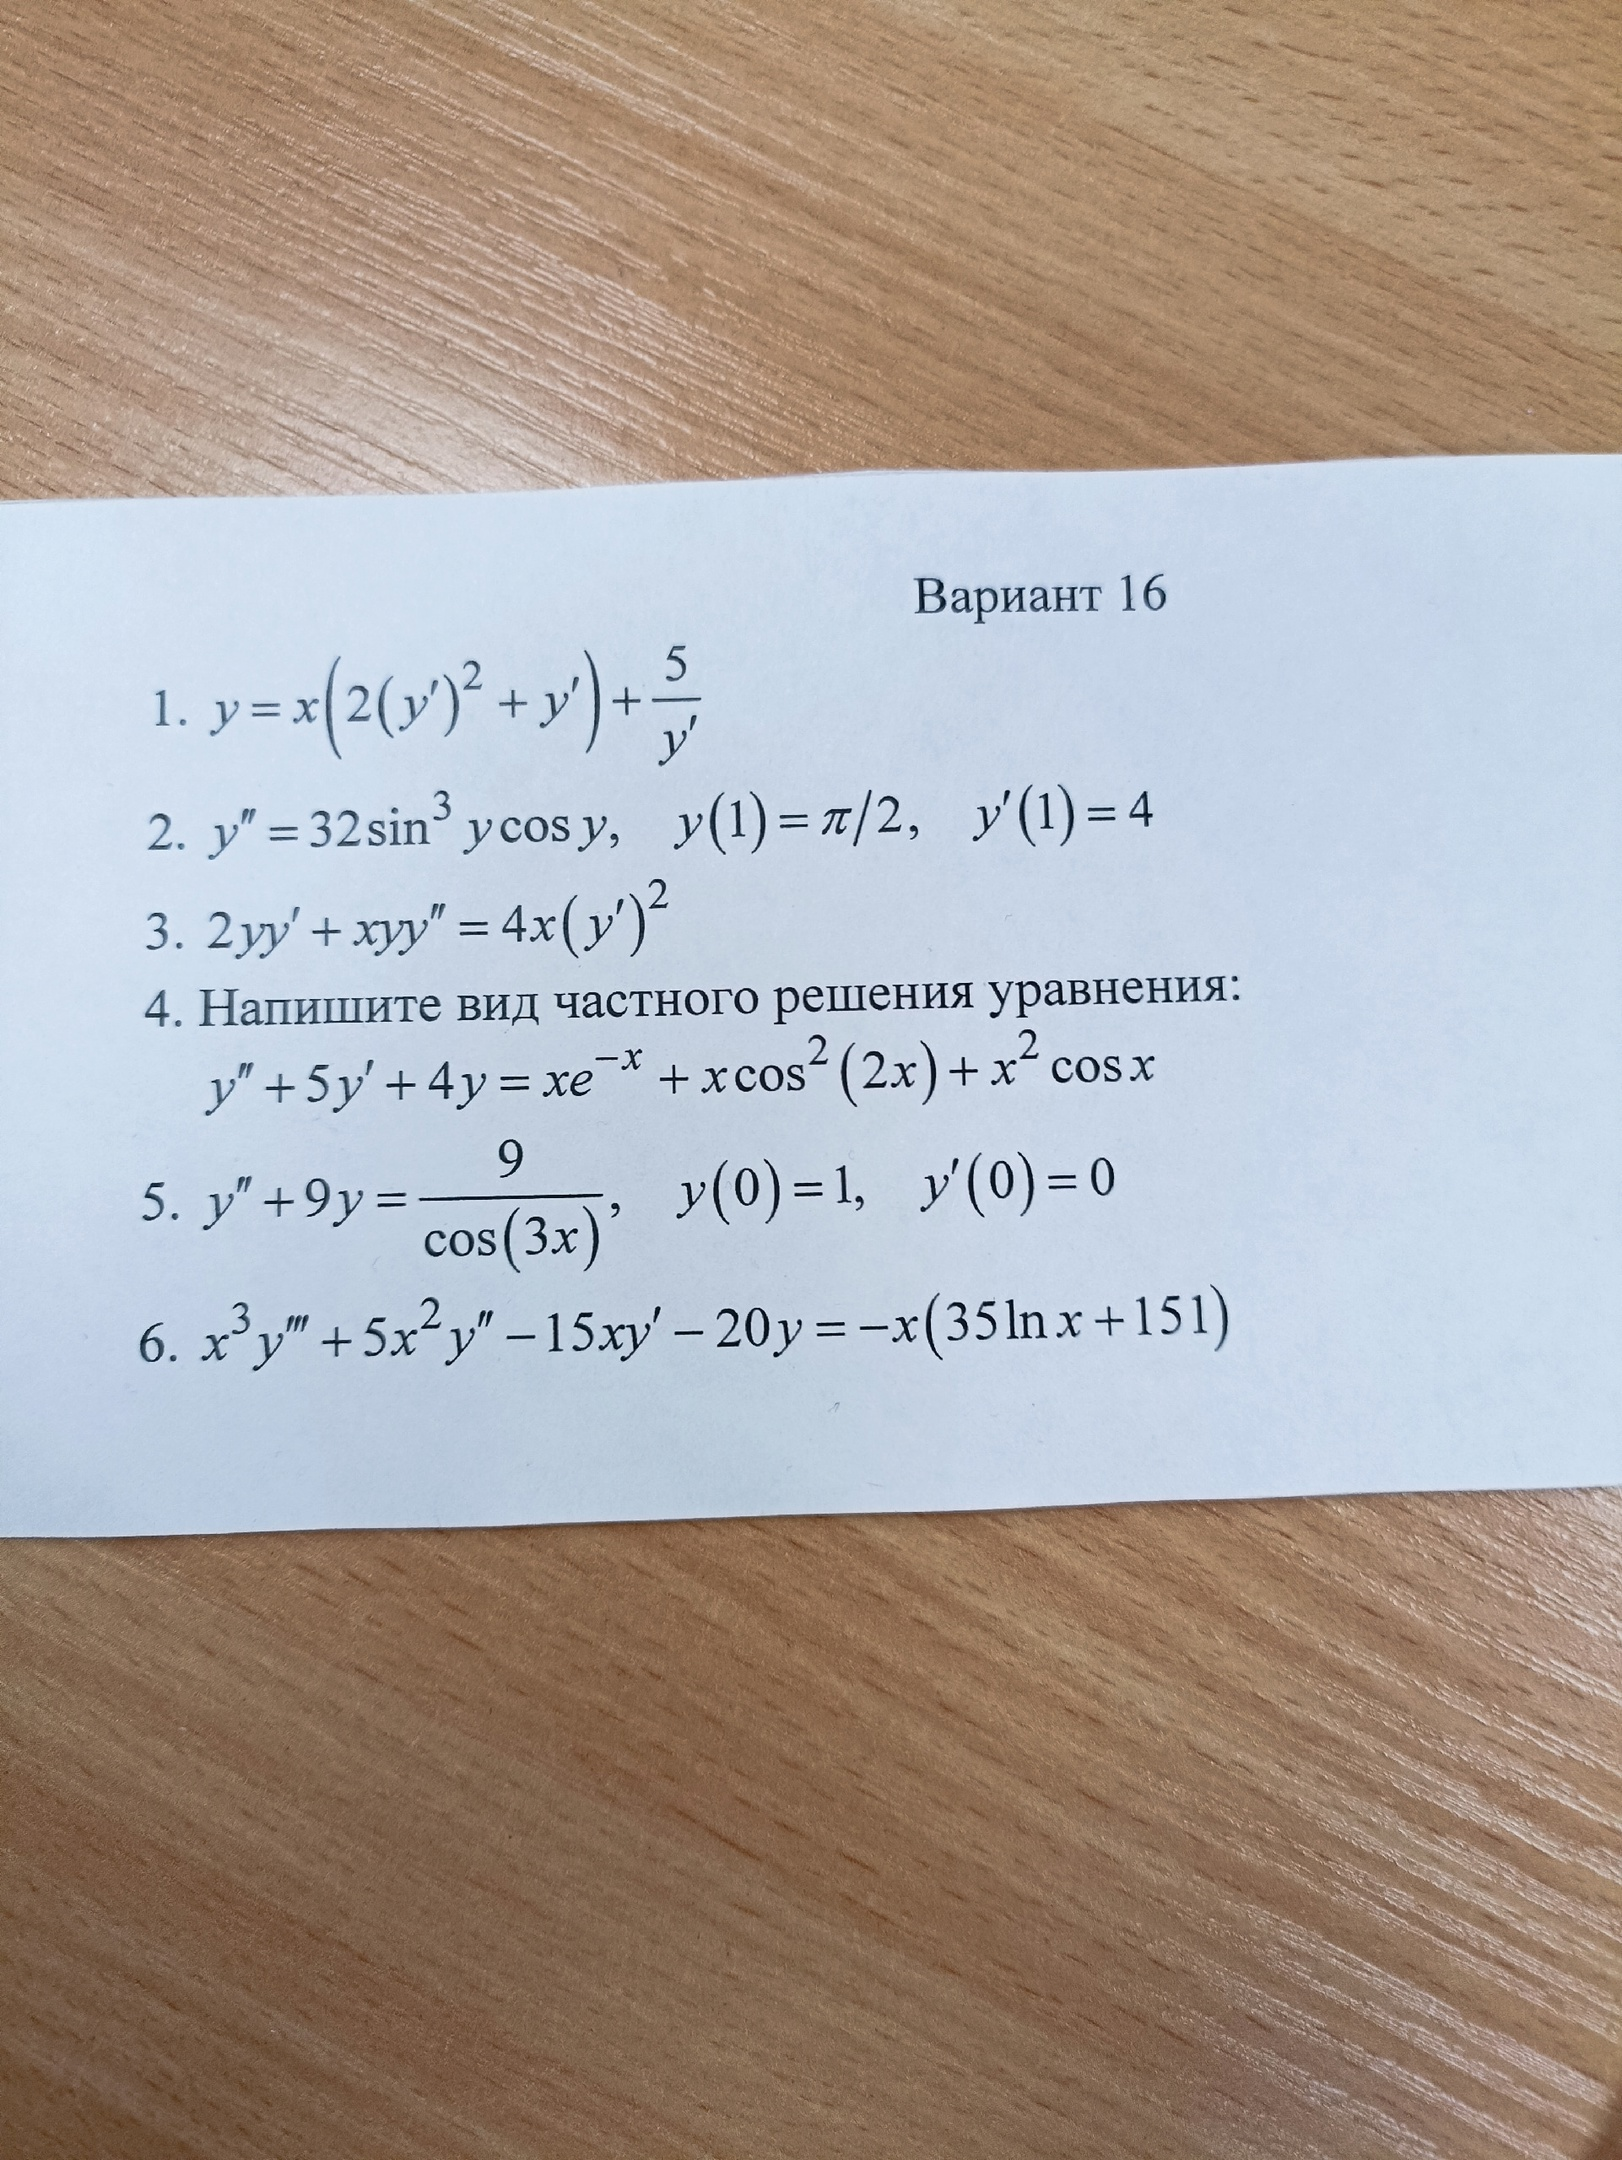
\includegraphics[width=0.65\textwidth]{PiSOb_S6Hes.jpeg}

    

    \begin{table}[h]
\caption{Замеры тестов на два потока}
%\label{tabular}
\begin{center}
\begin{tabular}{center}
№ & Количество ответов & время, сек. \\
1 & 2 & 60\\
2 & 10 & 72 \\
3 & 200 & 90 \\
\end{tabular}
\end{center}
\end{table}


 % \textbf{Вывод:} \\При некоторых типах входных данных получение нескольких ответов может быть незатруднительно

    

    
\section{Дальнейшие планы}
   % \begin{enumerate}
   %     \item 
   % \textbf{Имеем:}
   %  \\ Таблица с общим расписанием \\
   %  \textbf{Можно улучшить:}
   %  \\ Таблицы вида преподаватель/нагрузка, преподаватель/аудутория, группа/аудитория, аудитория/нагрузка
   %  \item \textbf{Имеем:} \\ Ручная запись данных в miniKanren \\ %\faCheck
   %  \textbf{Можно улучшить:} \\ Среда для работы с расписанием с помощью записи предметов в таблицы, запись требований в отдельные окна, а не в код %(хочу тут сказать, что можно сделать так, чтобы требования забивали не в код, а по-человечески в таблички всякие)
   %  \item
   %  \textbf{Имеем:}\\Получение нескольких ответов
   %  \\ \textbf{Можно улучшить:}\\ Возможность нахождения решения, удовлетворяющего "неформальным" запросам
   %  \item
   %  \textbf{Ограничения:}      
   %    \begin{enumerate}
   %    \item[\textcolor{blue}{\faCheck}] Полный учет учебного плана
   %        \item[\textcolor{blue}{\faCheck}] Не более 5 пар в день
   %        \item[\textcolor{blue}{\faCheck}]Проверка аудиторий на специализацию и вместимость
   %        \item[\textcolor{orange}{\faExclamation}] Добавить исключение окон
   %        \item [\textcolor{orange}{\faExclamation}]Невозможность поставить только одну пару за день
          
   %    \end{enumerate}      
   %  \end{enumerate}
    %\textbf{План решения дальнейших задач}
    
    Также была проделана работа по составлению плана и оценке сложности некоторых поставленных на следующий семестр задач
    \subsubsection{Отсутствие окон}
    В miniKanren каждой переменной сопоставляется некоторое особое число, называемое id. Каждой паре в расписании занятий соответствует некоторая переменная с уникальным id. При выводе программы можно сразу видеть, что переменная осталась "свежей", то есть она не имеет значение, что в нашем случае значит пустую пару. Но на этапе работы программы не так просто понять, является ли переменная свободной, или нет. Для реализации функции проверки на окна понадобится влезть в тело функции унификации и тд и тп
    \subsubsection{Одинокая пара}
    При решении вышепоставленной задачи решение этой задачи следует почти автоматически.

    Научившись проверять переменные на "пустоту", нам останется написать реляцию, которая, принимая расписание на день недели определенной группы , будет заканчивать провально при единственной непустой переменной, и успешно в остальных случаях.

    Также для двух этих задач важно помнить, что промежуточное решение удовлетворять им не должно, поэтому, помня специфику miniKanren, нужно будет ставить вызов реляций проверки на окна и одинокие пары в конце.
\subsubsection{Оценка расписания}
    Осмысленность данного пункта появляется благодаря поиску в ширину miniKanren, что также можно увидеть и на предыдущем слайде, где большее количество расписаний получается не намного дольше. 
     Как показано в статье ``Методика составления расписания уроков''`\cite{Методика} важно учитывать, в какие дни недели учащиеся более продуктивны, при каких сочетаниях предметов повышается утомляемость и тд и тп.

%\subsubsection{Возможность гарантированно занимать пару}



\section{Результаты}
\textbf{На данный момент выполнены следующие задачи:}
\begin{enumerate}
    \item Разработана процедура поиска расписания, соответствующее следующим требованиям
    \begin{itemize}
        \item Полный учет учебного плана
       % \item Не более 5 пар в день
        \item Проверка аудиторий на специализацию и вместимость
    \end{itemize}
    
    \item Разработано решение ручного визуализирования
\end{enumerate}

 \textbf{Код проекта} доступен в GitHub-репозитории: 
 
 \url{https://github.com/Azatic/Timetablenew}



% \section*{Заключение}
% % !TeX spellcheck = ru_RU
% !TEX root = vkr.tex

\textbf{Обязательно для промежуточного, полугодового, годового и  любых других отчётов.}

Кратко, что было сделано. Также здесь стоит писать задачи на будущее.

\textbf{Для практик/ВКР.} Также важно сделать список результатов, который будет один к одному соответствовать задачам из раздела~\ref{sec:task}.

\begin{itemize}
\item Результат к задаче 1 
\item Результат к задаче 2
\item и т.д.
\end{itemize}
\noindent Для промежуточных отчетов сюда важно записать какие задачи уже были сделаны за осенний семестр, а какие только планируется сделать.

Также сюда можно писать планы развития работы в будущем, или, если их много, выделять под это отдельную главу.



\setmonofont[Mapping=tex-text]{CMU Typewriter Text}
  \bibliographystyle{ugost2008ls}
  \bibliography{vkr}
\end{document}
